\subsection{Benchmarks and System}

We performed our evaluations on the MPI-based NAS Parallel Benchmarks (NPB)~\cite{nas}.
%
NPB includes four inputs sizes.
%
To keep the runtimes reasonable, we show results for the class \textit{B} (small-medium) and class \textit{C} (medium-large) inputs.
%

We compiled the NPB codes with the mpicc and mpif77 wrappers of MVAPICH 2.2.1, which are based on icc/ifort 14.0.2 using the prescribed -g and -O1 optimization flags.
%
Quick tests showed that higher optimization levels do not significantly improve the performance.
%

We ran all experiments on Comet at the San Diego Supercomputer Center~\cite{comet}, whose filesystem is NFS and Lustre.
%
Comet has 1944 compute nodes, each of which has dual-socket Intel Xeon E5-2680 v3 processors with a total of 28 cores (14 per socket) and 128 GB of main memory.
%
Note that we only used 16 cores per node as many of the NPB programs require a core count that is a power of two.
%
To study the scaling behavior, we ran experiments on 1, 4, 16 and 64 compute nodes, i.e., on up to 1024 cores.

\subsection{Metrics}

We use the following metrics to quantify and compare the performance of the tracing tools.
%
Unless otherwise noted, all results are based on the median of three identical experiments.
%
\begin{itemize}
\item The \textbf{tracing overhead} is the runtime of the target application when it is being traced divided by the runtime of the same application without tracing.
%
This lower-is-better ratio measures by how much the tracing (and the compression when enabled) slows down the target application.
%
\item The \textbf{tracing bandwidth} is the size of the trace information divided by the application runtime.
%
To make the results easier to compare, we generally list the tracing bandwidth per core, i.e., the tracing bandwidth divided by the number of cores used.
%
This lower-is-better metric is expressed in kilobytes per second (kB/s) per core.
%
It specifies the average needed bandwidth to record the trace data.
%
\item The \textbf{compression ratio} is the size of the uncompressed trace divided by the size of the generated (compressed) trace.
%
This higher-is-better ratio measures the factor by which the compression reduces the trace size.
%
In other words, without compression, the tracing bandwidth would be higher by this factor.
\end{itemize}

\subsection{Tracing Tools}
\label{sec:tracing-tools}

We compare our \parlot tool, implemented on top of \pin 3.5, with \callgrind 3.13.
%
\parlot was compiled with gcc 4.9.2 using \pin 's make system and \callgrind with Valgrind's make system.
%
We created the following versions of \parlot to evaluate different aspects of its design.

% ORIGINAL TABLE
\iffalse
\begin{table*}[]
\caption{Overhead added by each tool. Last column is the geometric mean}
\label{comet_sd_pMpAcg_BC_itn_p3.5}\begin{center}
\npdecimalsign{.}
\nprounddigits{1}
\begin{tabular}{lrrrrrrrrr}
\hline
                &   bt &   cg &    ep &    ft &   is &   lu &   mg &   sp &   GM \\
\hline
 pinMain.B.1    & 1.55 & 1.82 &  2.62 &  2.11 & 2.47 & 1.31 & 2.53 & 1.33 & 1.90 \\
 pinMain.B.4    & 1.76 & 1.85 &  1.89 &  1.74 & 1.78 & 1.77 & 1.52 & 1.73 & 1.75 \\
 pinMain.B.16   & 2.15 & 2.58 &  1.99 &  1.89 & 1.78 & 2.73 & 2.43 & 2.15 & 2.19 \\
 pinMain.B.64   & 2.10 & 2.17 &  2.39 &  1.96 & 4.31 & 4.39 & 1.97 & 2.07 & 2.52 \\
 AVG            & 1.89 & 2.10 &  2.22 &  1.92 & 2.58 & 2.55 & 2.11 & 1.82 & 2.09 \\
 pinAll.B.1     & 1.84 & 2.73 &  4.18 &  2.78 & 4.22 & 1.73 & 4.75 & 1.72 & 2.77 \\
 pinAll.B.4     & 2.57 & 3.06 &  3.41 &  2.77 & 2.96 & 2.76 & 2.79 & 2.66 & 2.86 \\
 pinAll.B.16    & 3.52 & 4.20 &  3.39 &  2.94 & 2.83 & 4.30 & 4.46 & 3.65 & 3.62 \\
 pinAll.B.64    & 3.14 & 3.26 &  3.83 &  3.02 & 5.44 & 4.65 & 3.17 & 3.31 & 3.65 \\
 AVG            & 2.77 & 3.31 &  3.70 &  2.88 & 3.86 & 3.36 & 3.79 & 2.83 & 3.23 \\
 callgrind.B.1  & 8.62 & 5.96 &  8.92 & 10.14 & 2.52 & 7.54 & 3.27 & 6.61 & 6.10 \\
 callgrind.B.4  & 6.02 & 3.60 &  2.90 &  3.50 & 1.46 & 5.18 & 1.24 & 5.78 & 3.23 \\
 callgrind.B.16 & 4.28 & 3.26 &  2.24 &  2.17 & 1.70 & 4.62 & 1.81 & 4.34 & 2.84 \\
 callgrind.B.64 & 2.26 & 2.03 &  1.66 &  2.05 & 4.07 & 3.97 & 1.47 & 2.46 & 2.34 \\
 AVG            & 5.29 & 3.71 &  3.93 &  4.46 & 2.44 & 5.33 & 1.95 & 4.80 & 3.63 \\
 pinMain.C.1    & 1.41 & 1.29 &  2.51 &  1.89 & 2.29 & 1.12 & 1.74 & 1.10 & 1.60 \\
 pinMain.C.4    & 1.58 & 1.73 &  1.75 &  1.62 & 1.68 & 1.33 & 1.81 & 1.35 & 1.60 \\
 pinMain.C.16   & 1.82 & 2.38 &  2.46 &  1.51 & 1.80 & 2.18 & 2.36 & 1.80 & 2.01 \\
 pinMain.C.64   & 2.23 & 2.74 &  2.39 &  1.59 & 4.46 & 3.42 & 2.43 & 2.24 & 2.57 \\
 AVG            & 1.76 & 2.04 &  2.28 &  1.65 & 2.56 & 2.01 & 2.08 & 1.62 & 1.94 \\
 pinAll.C.1     & 1.47 & 1.55 &  3.17 &  1.97 & 2.82 & 1.23 & 2.52 & 1.19 & 1.87 \\
 pinAll.C.4     & 1.89 & 2.42 &  2.56 &  2.06 & 2.56 & 1.70 & 3.08 & 1.71 & 2.20 \\
 pinAll.C.16    & 2.69 & 3.47 &  4.07 &  2.14 & 2.80 & 3.18 & 3.98 & 2.54 & 3.04 \\
 pinAll.C.64    & 3.61 & 4.13 &  4.21 &  2.22 & 5.47 & 4.43 & 4.23 & 3.02 & 3.80 \\
 AVG            & 2.42 & 2.89 &  3.50 &  2.10 & 3.41 & 2.63 & 3.45 & 2.11 & 2.73 \\
 callgrind.C.1  & 8.50 & 4.44 & 13.18 & 13.13 & 3.32 & 7.90 & 5.91 & 5.14 & 6.91 \\
 callgrind.C.4  & 8.66 & 4.46 &  4.76 &  6.37 & 1.65 & 6.38 & 2.75 & 6.34 & 4.64 \\
 callgrind.C.16 & 6.86 & 3.91 &  3.11 &  2.76 & 1.79 & 6.40 & 2.14 & 6.09 & 3.69 \\
 callgrind.C.64 & 4.37 & 3.46 &  2.13 &  2.50 & 4.24 & 5.24 & 2.08 & 3.81 & 3.30 \\
 AVG            & 7.10 & 4.07 &  5.79 &  6.19 & 2.75 & 6.48 & 3.22 & 5.34 & 4.63 \\
\hline
\end{tabular}
\npnoround
\end{center}
\end{table*}
\fi



\iftrue

\begin{table*}[!b]
\caption{Overhead added by each tool}
\label{comet_sd_pMpAcg_BC_itn_p3.5}\begin{center}
\npdecimalsign{.}
\nprounddigits{1}
\scalebox{0.90}{
\begin{tabular}{|c|c|c|n{2}{1}n{2}{1}n{2}{1}n{2}{1}n{2}{1}n{2}{1}n{2}{1}n{2}{1}|n{2}{1}|}
\hline
Input & Tool & \# Nodes  & \multicolumn{1}{c}{bt} & \multicolumn{1}{c}{cg} & \multicolumn{1}{c}{ep} & \multicolumn{1}{c}{ft} & \multicolumn{1}{c}{is} & \multicolumn{1}{c}{lu} & \multicolumn{1}{c}{mg} & \multicolumn{1}{c|}{sp} & \multicolumn{1}{c|}{GM} \\ \hline
\multirow{15}{*}{B} & \multirow{5}{*}{\parlotm} & 1 & 1.55 & 1.82 &  2.62 &  2.11 & 2.47 & 1.31 & 2.53 & 1.33 & 1.90 \\
 &  & 4  & 1.76 & 1.85 &  1.89 &  1.74 & 1.78 & 1.77 & 1.52 & 1.73 & 1.75 \\
 &  & 16  & 2.15 & 2.58 &  1.99 &  1.89 & 1.78 & 2.73 & 2.43 & 2.15 & 2.19 \\
 &  & 64  & 2.10 & 2.17 &  2.39 &  1.96 & 4.31 & 4.39 & 1.97 & 2.07 & 2.52 \\ \cline{3-12} 
 &  & AVG & 1.89 & 2.10 &  2.22 &  1.92 & 2.58 & 2.55 & 2.11 & 1.82 & 2.09 \\ \cline{2-12} 
 & \multirow{5}{*}{\parlota} & 1 & 1.84 & 2.73 &  4.18 &  2.78 & 4.22 & 1.73 & 4.75 & 1.72 & 2.77 \\
 & & 4     & 2.57 & 3.06 &  3.41 &  2.77 & 2.96 & 2.76 & 2.79 & 2.66 & 2.86 \\
 & & 16    & 3.52 & 4.20 &  3.39 &  2.94 & 2.83 & 4.30 & 4.46 & 3.65 & 3.62 \\
 & & 64    & 3.14 & 3.26 &  3.83 &  3.02 & 5.44 & 4.65 & 3.17 & 3.31 & 3.65 \\ \cline{3-12} 
 & & AVG   & 2.77 & 3.31 &  3.70 &  2.88 & 3.86 & 3.36 & 3.79 & 2.83 & {\boldmath}3.23 \\ \cline{2-12} 
 & \multirow{5}{*}{\callgrind}  & 1  & 8.62 & 5.96 &  8.92 & 10.14 & 2.52 & 7.54 & 3.27 & 6.61 & 6.10 \\
 & & 4   & 6.02 & 3.60 &  2.90 &  3.50 & 1.46 & 5.18 & 1.24 & 5.78 & 3.23 \\
 & & 16  & 4.28 & 3.26 &  2.24 &  2.17 & 1.70 & 4.62 & 1.81 & 4.34 & 2.84 \\
 & & 64  & 2.26 & 2.03 &  1.66 &  2.05 & 4.07 & 3.97 & 1.47 & 2.46 & 2.34 \\ \cline{3-12} 
 & & AVG & 5.29 & 3.71 &  3.93 &  4.46 & 2.44 & 5.33 & 1.95 & 4.80 & {\boldmath}3.63 \\ \hline
 \multirow{15}{*}{C} & \multirow{5}{*}{\parlotm} & 1  & 1.41 & 1.29 &  2.51 &  1.89 & 2.29 & 1.12 & 1.74 & 1.10 & 1.60 \\
 & & 4   & 1.58 & 1.73 &  1.75 &  1.62 & 1.68 & 1.33 & 1.81 & 1.35 & 1.60 \\
 & & 16  & 1.82 & 2.38 &  2.46 &  1.51 & 1.80 & 2.18 & 2.36 & 1.80 & 2.01 \\
 & & 64  & 2.23 & 2.74 &  2.39 &  1.59 & 4.46 & 3.42 & 2.43 & 2.24 & 2.57 \\ \cline{3-12} 
 & & AVG & 1.76 & 2.04 &  2.28 &  1.65 & 2.56 & 2.01 & 2.08 & 1.62 & {\boldmath}1.94 \\ \cline{2-12} 
 & \multirow{5}{*}{\parlota} & 1 & 1.47 & 1.55 &  3.17 &  1.97 & 2.82 & 1.23 & 2.52 & 1.19 & 1.87 \\
 & & 4   & 1.89 & 2.42 &  2.56 &  2.06 & 2.56 & 1.70 & 3.08 & 1.71 & 2.20 \\
 & & 16  & 2.69 & 3.47 &  4.07 &  2.14 & 2.80 & 3.18 & 3.98 & 2.54 & 3.04 \\
 & & 64  & 3.61 & 4.13 &  4.21 &  2.22 & 5.47 & 4.43 & 4.23 & 3.02 & 3.80 \\ \cline{3-12}
 & & AVG & 2.42 & 2.89 &  3.50 &  2.10 & 3.41 & 2.63 & 3.45 & 2.11 & {\boldmath}2.73 \\ \cline{2-12} 
 & \multirow{5}{*}{\callgrind} & 1 & 8.50 & 4.44 & 13.18 & 13.13 & 3.32 & 7.90 & 5.91 & 5.14 & 6.91 \\
 & & 4   & 8.66 & 4.46 &  4.76 &  6.37 & 1.65 & 6.38 & 2.75 & 6.34 & 4.64 \\
 & & 16  & 6.86 & 3.91 &  3.11 &  2.76 & 1.79 & 6.40 & 2.14 & 6.09 & 3.69 \\
 & & 64  & 4.37 & 3.46 &  2.13 &  2.50 & 4.24 & 5.24 & 2.08 & 3.81 & 3.30 \\ \cline{3-12}
 & & AVG & 7.10 & 4.07 &  5.79 &  6.19 & 2.75 & 6.48 & 3.22 & 5.34 & {\boldmath}4.63 \\ \hline
\end{tabular}}
\npnoround
\end{center}
\end{table*}

\fi



\begin{itemize}
\item \textbf{\parlotm} is the normal \parlot tool configured to only collect function-call traces from the main image of the application.
\item \textbf{\parlota} is the normal \parlot tool configured to collect function-call traces from all images of the application, including library function calls.
\item \textbf{\pininit} is a crippled version of \parlot from which the tracing code has been removed.
%
The purpose of \pininit is to see how much of the overhead is due to \pin.
\item \textbf{\parlotnc} is the normal \parlot tool but with compression disabled.
%
It writes out the captured data in uncompressed form.
%
The purpose of \parlotnc is to show the performance impact of the compression.
\end{itemize}

It proved surprisingly difficult to find a tool that is similar to \parlot because there appear to be no other tools that generate whole program call trace.
%
In the end, we settled on \callgrind as the most similar tool we could find and used it for our comparisons.
%
\callgrind is based on the Valgrind DBI tool.
%
It collects function-call graphs combined with performance data to show the user what portion of the execution time has been spent in each function.

%%%%%%%%%%%%%%%%%%%%%%%%%%%%%%%%%
% FROM RESULTS - average overhead
%%%%%%%%%%%%%%%%%%%%%%%%%%%%%%%%%

Each \callgrind trace file contains a sequence of function names (or their code) plus numerical data for each function on its caller-callee relationship with other functions.
%
Moreover, it contains cost information for each function in terms of how many machine instructions it read.
%
This information is collected using hardware performance counters.
%
The format of the file is plain ASCII text.
%
Interestingly, all numerical values are expressed relative to previous values, i.e., they are delta (or difference) encoded.
%
This simple form of compression is enabled by default in \callgrind.


\begin{figure}[t]
\centering
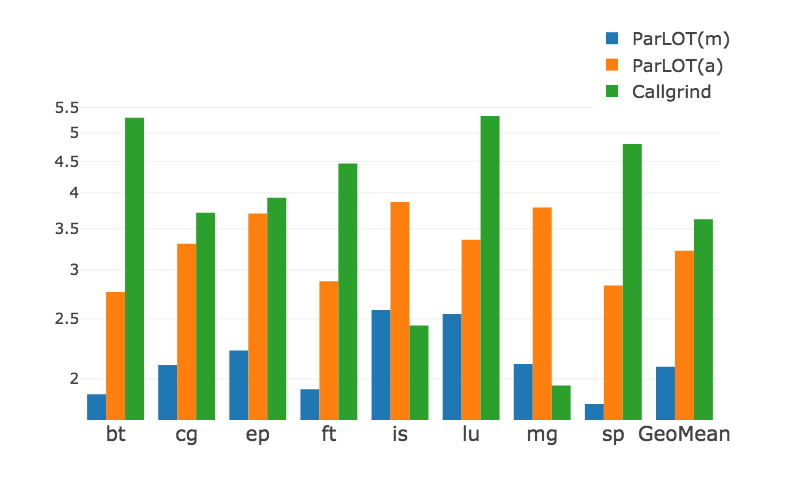
\includegraphics[width=3.4in,height=1.9in]{figs.comet.newMed/comet_chartAvg_sd_B_p3_5.png}
\caption{Average tracing overhead on the NPB applications - Input B}
\label{comet_chartAvg_sd_B_p3_5}
\end{figure}

\begin{figure}[t]
\centering
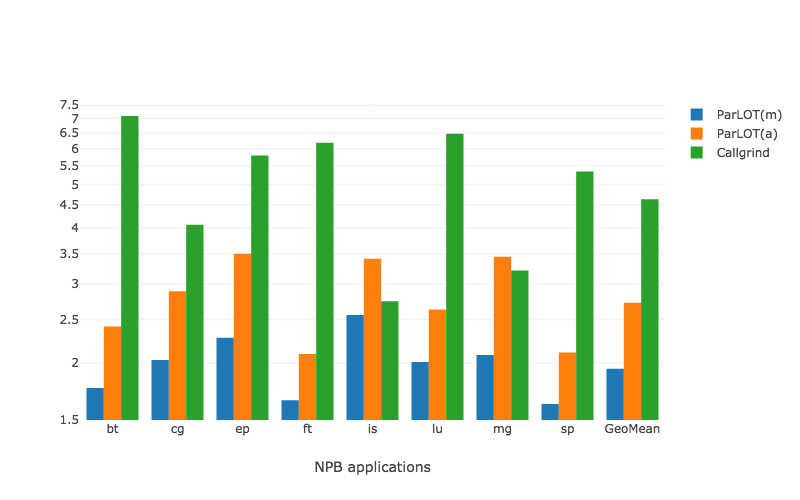
\includegraphics[width=3.4in,height=1.9in]{figs.comet.newMed/comet_chartAvg_sd_C_p3_5.png}
\caption{ Average tracing overhead on the NPB applications - Input C}
\label{comet_chartAvg_sd_C_p3_5}
\end{figure}


We believe the information traced by \callgrind is reasonably similar to the information traced by \parlotm.
%
Whereas \callgrind 's traces include performance data that \parlot does not capture, \parlot records the whole-program call trace, which \callgrind does not capture.
%
The full function-call trace is a strict superset of the call-graph information that \callgrind records because the call graph can be extracted from the function-call trace but not vice versa.
%
In particular, \callgrind cannot recreate the order of the function calls a thread made whereas \parlot can.


